\subsubsection{Repetition code}
For this error code information is encoded by repeating the 
intended message some amount of times, and then decoding it
by performing a majority vote on the transmitted message.


\begin{figure}[h!]
	\begin{center}
	\captionsetup{justification=centering,margin=2cm}
	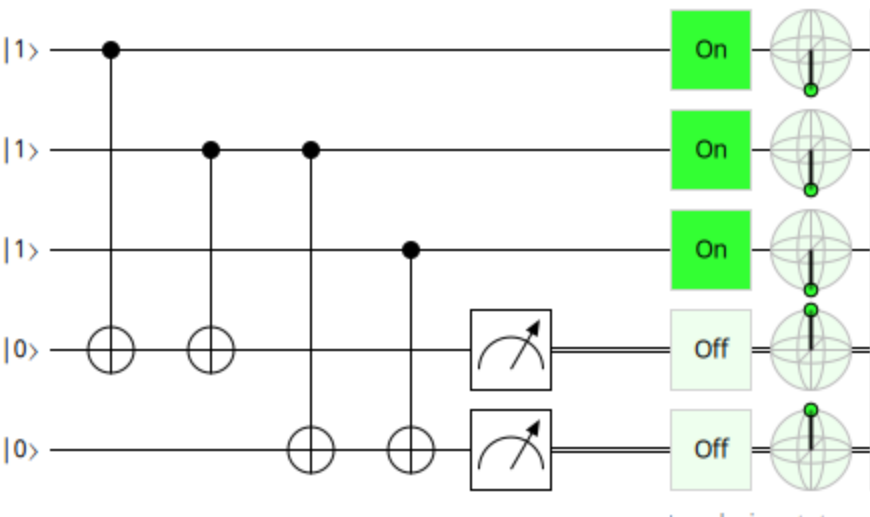
\includegraphics[scale=0.2]{./img/figures/bitflipSyndromeExtraction3Rep.png}\\
	\caption{Bitflip Syndrome extractor for [[3,1,$\frac{1}{2}$]] repetition code\\
        +1 measurement result on first ancilla indicates a bitflip error
        on qubits 1 or 2, +1 result on second ancilla indicates 
		bitflip on second or third qubit}
	\label{fig: syndrome extractor}
	\end{center}
\end{figure}

A quantum equivalent of the 3-bit repetition code performed on
the message $|1\rangle$ is the [[3,1,$\frac{1}{2}$]] repetition
code depicted in 
Figure~\ref{fig: syndrome extractor}
, including so-called
$syndrome\ extraction$. A syndrome is a stabilizer that can be
measured to detect whether and where an error has occurred
in a multi-qubit system. It is crucial that the 
measurement of such syndromes occurs without harming the actual
quantum information stored in the $data-qubits$. Therefore
two additional \emph{ancilla-qubits} (both initialized to 
$|0\rangle$) are attached to the circuit via CNOTs.
This circuit is stabilized by IZZ and ZZI, measured by ancilla 
1 and 2. The measurement result will therefore be a vector of length
two, with each entry either being +1 or -1. To simplify the 
algebra this will be changed to the binary representation of 0 
for +1 and 1 for -1. 

To represent the code, stabilizers can be stacked together to
a so-called parity-check-matrix, which satisfies:
\begin{equation}\label{eq: pcm}
	M_{pc}\cdot \vec{v}_{error} = \vec{v}_{syndrome}
\end{equation}
So e.g. the parity check matrix for the $[3,1,\frac{1}{2}]$
repetition code would be:

\begin{equation}
	M_{pc3} = \left( 
	\begin{array}{ccc}
		1 & 1 & 0 \\
		0 & 1 & 1
	\end{array}
	\right)
\end{equation}
And the syndrome for an X error on the first qubit would be
$\left(\begin{array}{c}1\\0\end{array}\right)$.

If we draw a graph to represent this code, with here square nodes being
 ancilla qubits
and round nodes being data qubits, we obtain the following:

\begin{figure}[h!]
	\begin{center}
	\captionsetup{justification=centering,margin=2cm}
	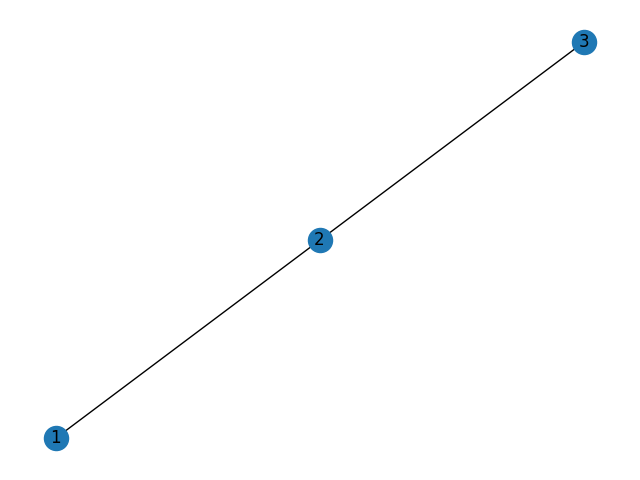
\includegraphics[scale=0.4]{./img/figures/rep_3_graph.png}\\
	\caption{Graph for [[3,1,$\frac{1}{2}$]] repetition code with error on
    node 1 marked in green and resulting syndrome marked red.
    Squares represent ancilla qubits and circles represent data qubits.}
        
	\label{fig: rep_graph}
	\end{center}
\end{figure}
